\documentclass[11pt,a4paper]{article}
\usepackage[T1]{fontenc}
\usepackage{lmodern}
\usepackage[spanish]{babel}
\usepackage[margin=2.5cm]{geometry}
\usepackage{booktabs,tabularx,graphicx,hyperref,enumitem,parskip}
\hypersetup{hidelinks}
\setlength{\parskip}{0.6em}
\begin{document}

{\LARGE\bfseries Proyecto final: clasificación visual de productos para Lokora\par}\vspace{0.4em}
\noindent \textbf{Avance I (R2-A3-S11). Definición del problema}\par
\noindent Universidad de Cundinamarca. Posgrado. Aplicaciones en Deep Learning (608145)\par
\noindent Docente: Wilson Mauro Rojas Reales\par
\noindent Estudiante: Harold Duque (trabajo individual)\par
\noindent Fecha: 17 de noviembre de 2026\par
\section*{Resumen}
\noindent Se propone una extensión de Lokora, una plataforma de comercio desarrollada en la hackatón de Open Payments (Medellín, 16 y 17 de octubre de 2026), que sugiere la categoría de un producto a partir de su fotografía. El vendedor confirma o corrige la sugerencia antes de guardar. La solución usa MobileNetV2 con aprendizaje por transferencia y se compara con dos referencias sencillas. Este documento define el problema, revisa cinco trabajos y describe el diseño de la solución. Los resultados experimentales se presentan en el Avance III.\par
\section*{Avance I. Definición del problema}
\subsection*{1. Contexto real y problema}
\noindent Un comercio que publica productos en Lokora debe cargar fotografía, descripción y categoría de cada referencia. Cuando la categoría se asigna a mano, el tiempo de publicación crece con el número de productos y pueden aparecer criterios inconsistentes entre vendedores. La aplicación ya almacena una categoría por producto y administra sus imágenes, lo que permite incorporar una asistencia visual durante la carga.\par
\noindent \textbf{Aplicación original.} Video de la aplicación de Lokora en funcionamiento: \url{https://youtube.com/shorts/1stYAlFeCe8}\par
\noindent \textbf{Pregunta de investigación.} ?`Puede un modelo de clasificación de imágenes sugerir correctamente una de tres categorías (frutas, verduras, envasados) con calidad suficiente para ayudar al vendedor?\par
\noindent \textbf{Alcance.} Una fotografía con un producto principal y tres categorías. Panadería, artesanías, experiencias y productos mixtos se registran manualmente. La clasificación no interviene en pagos.\par
\noindent \textbf{Cómo se mide el impacto.} El proyecto debe poder medir el efecto, como pidió el docente. Se compararán el tiempo de carga manual y asistida y la tasa de correcciones del vendedor. Este ahorro no está medido todavía y no se afirma un porcentaje.\par
\noindent \textbf{Disponibilidad de datos.} Hay datos históricos públicos (Grocery Store Dataset) para entrenar. Las fotografías propias de comercios de Lokora no existen aún; se recolectarán después para medir el cambio de dominio.\par
\subsection*{2. Objetivos}
\noindent \textbf{General.} Diseñar y evaluar una extensión reproducible de clasificación visual para Lokora, comparando MobileNetV2 con referencias sencillas.\par
\noindent \textbf{Específicos.}\par
\begin{enumerate}[nosep]
\item Preparar un conjunto con etiquetas, procedencia y particiones fijas.
\item Comparar modelos con macro-F1 y errores por clase.
\item Registrar datos, código, parámetros y modelos de cada ejecución.
\item Definir el flujo en que el vendedor confirma la sugerencia.
\item Medir en un piloto el tiempo de carga y las correcciones.
\end{enumerate}
\subsection*{3. Revisión de literatura y análisis comparativo}
\noindent Se revisaron cinco trabajos. Los datos bibliográficos se verificaron en arXiv. Las descripciones se basan en los resúmenes de los artículos, no en una lectura completa; las cifras de resultados de cada uno deben citarse del texto original antes de la entrega final.\par
\begin{center}\small
\begin{tabularx}{\textwidth}{XXXX}
\toprule
\textbf{Trabajo} & \textbf{Aporte} & \textbf{Datos y entrada} & \textbf{Relación con Lokora} \\
\midrule
Klasson, Zhang y Kjellström (2019). \emph{A Hierarchical Grocery Store Image Dataset with Visual and Semantic Labels}. WACV. & Conjunto de fotografías de frutas, verduras y lácteos y jugos refrigerados tomadas con smartphone en 18 tiendas; 46 clases gruesas y etiquetas jerárquicas. & Imágenes naturales de tienda & Es la fuente de datos del piloto. Su dominio (fotos de teléfono en tienda) se parece al de un vendedor, pero no es el de Lokora. \\
Sandler et al. (2018). \emph{MobileNetV2: Inverted Residuals and Linear Bottlenecks}. CVPR. & Arquitectura móvil eficiente con bloques residuales invertidos y cuellos de botella lineales. & Imágenes de 224 $\times$ 224 & Es el modelo elegido: pequeño, rápido y apto para servir sugerencias con baja latencia. \\
Tan y Le (2019). \emph{EfficientNet: Rethinking Model Scaling for Convolutional Neural Networks}. ICML. & Escalado compuesto de profundidad, ancho y resolución. & Imágenes de resolución variable & Alternativa de mayor precisión y mayor costo. Se deja como mejora futura si MobileNetV2 resulta insuficiente. \\
Zahavy et al. (2016). \emph{Is a picture worth a thousand words? A Deep Multi-Modal Fusion Architecture for Product Classification in e-commerce}. & Fusión de texto e imagen para clasificar productos de comercio electrónico con muchas categorías. & Imagen y título del producto & Muestra que el texto aporta información. Lokora tiene nombre y descripción del producto, así que se propone como extensión. \\
Gross et al. (2025). \emph{Cross-Platform E-Commerce Product Categorization and Recategorization: A Multimodal Hierarchical Classification Approach}. & Clasificación multimodal y jerárquica con RoBERTa, ViT y CLIP sobre 271.700 productos de 40 plataformas. & Imagen y texto & Respalda el uso de imagen y texto y la jerarquía de categorías; su escala excede la de este piloto. \\
\bottomrule
\end{tabularx}
\end{center}
\noindent \textbf{Análisis comparativo.} Los dos primeros trabajos definen el piloto: datos de fotos reales en tienda y un modelo liviano. EfficientNet ofrece más capacidad a mayor costo, y la decisión entre ambos debe tomarse con la validación, no por preferencia. Los dos trabajos de comercio electrónico usan imagen y texto, con muchas más categorías y datos que este proyecto. Por eso el piloto parte solo de imagen y tres clases, y la fusión con texto queda como evolución.\par
\subsection*{4. Diseño de la solución}
\noindent \textbf{Modelo.} MobileNetV2 preentrenada en ImageNet, con la base congelada y una cabeza nueva: pooling global, dropout de 0,2 y capa softmax de tres salidas. Optimizador Adam (tasa 0,001), lotes de 32, máximo 20 épocas y parada temprana tras cuatro épocas sin mejora en la pérdida de validación. Son valores iniciales, no resultado de una búsqueda.\par
\noindent \textbf{Referencias de comparación.} (a) predecir siempre la clase más frecuente; (b) regresión logística sobre 54 atributos de histograma de color RGB. Si la red no supera estas referencias en validación, no se justifica usarla.\par
\noindent \textbf{Métrica principal.} Macro-F1, porque da el mismo peso a las tres clases. También exactitud, precisión y recall por clase, matriz de confusión y latencia. Meta exploratoria de macro-F1 de prueba $\geq$ 0,80, que no es un resultado alcanzado.\par
\noindent \textbf{Herramientas.} Python, TensorFlow/Keras, scikit-learn, Google Colab para el entrenamiento, GitHub para el código.\par
\noindent \textbf{Arquitectura de integración.} La figura 1 distingue la aplicación original (React y Express) del servicio de inferencia en Python propuesto. El servicio expone \texttt{POST /predict-category}, recibe una imagen (hasta 5 MB) y devuelve categoría, puntuaciones, versión y tiempo. El vendedor confirma desde la interfaz antes de guardar; si el servicio no responde, se registra manualmente.\par
\begin{figure}[htbp]\centering
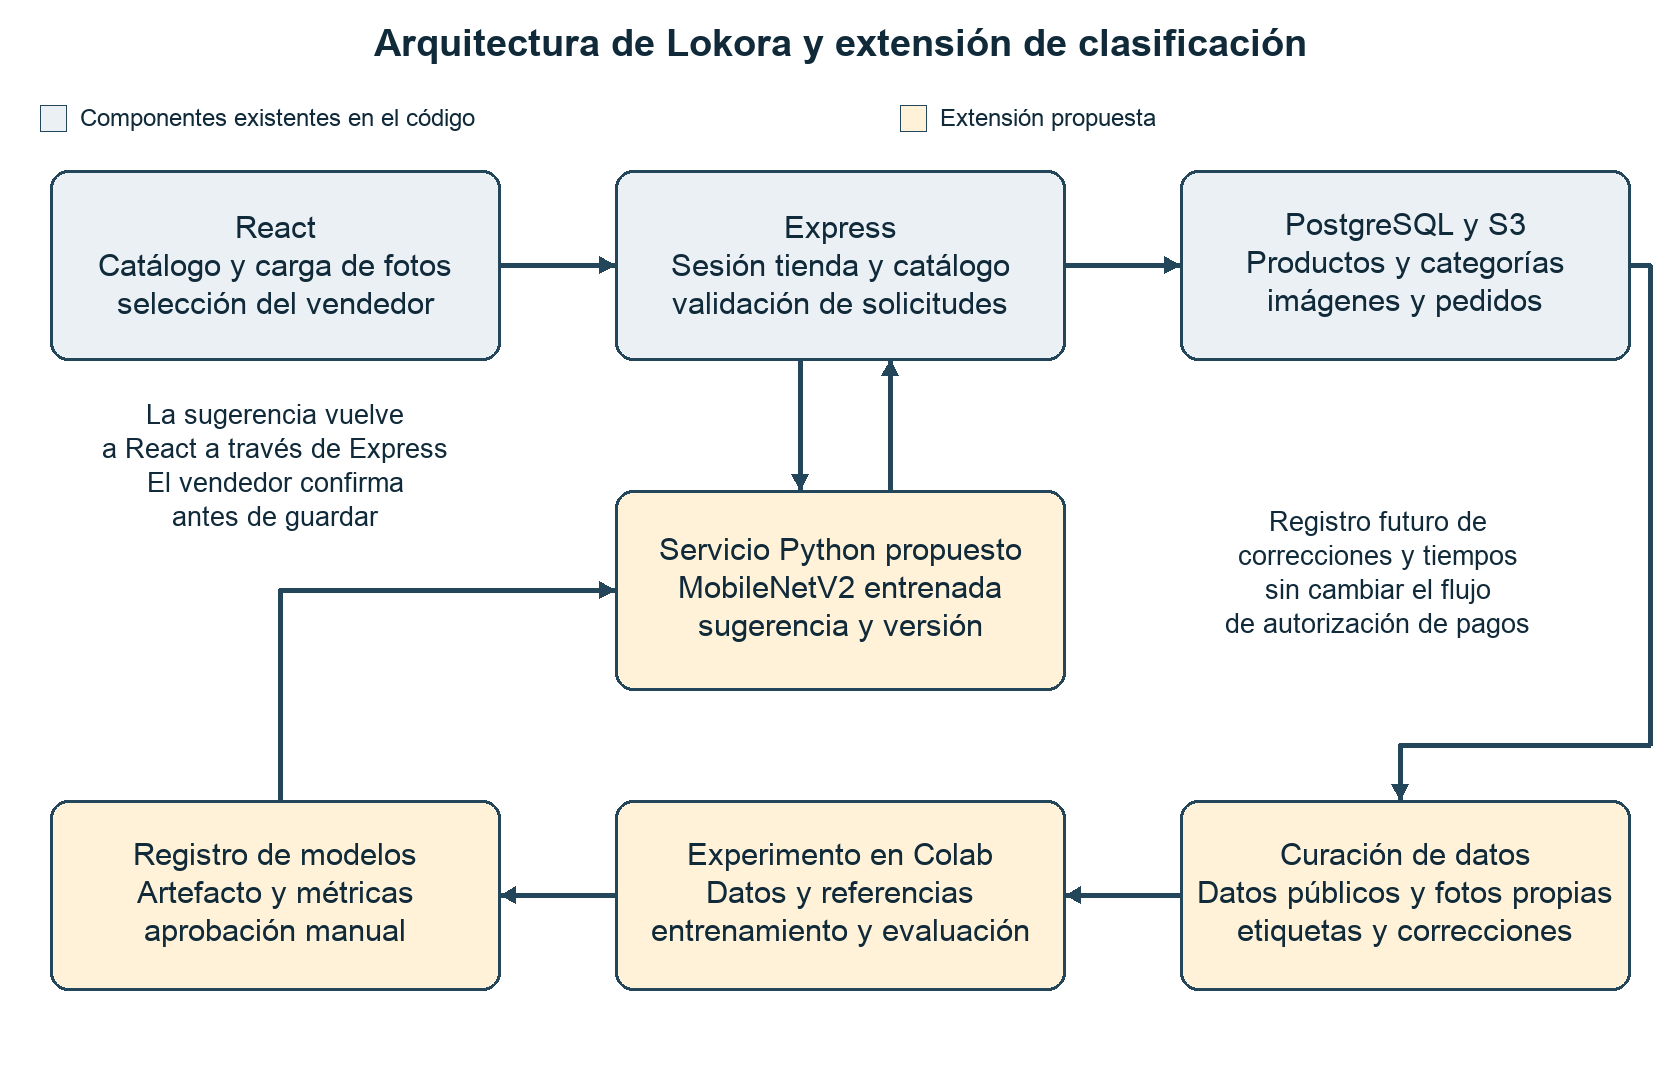
\includegraphics[width=0.92\textwidth]{figuras/bloques_lokora.png}\par\vspace{0.4em}
{\small Figura 1. Arquitectura de Lokora y extensión propuesta\par}
\end{figure}
\subsection*{Referencias}
\noindent [1] Klasson, M., Zhang, C. y Kjellström, H. (2019). A Hierarchical Grocery Store Image Dataset with Visual and Semantic Labels. IEEE Winter Conference on Applications of Computer Vision (WACV). \url{https://arxiv.org/abs/1901.00711}\par
\noindent [2] Sandler, M., Howard, A., Zhu, M., Zhmoginov, A. y Chen, L.-C. (2018). MobileNetV2: Inverted Residuals and Linear Bottlenecks. CVPR. \url{https://arxiv.org/abs/1801.04381}\par
\noindent [3] Tan, M. y Le, Q. V. (2019). EfficientNet: Rethinking Model Scaling for Convolutional Neural Networks. ICML. \url{https://arxiv.org/abs/1905.11946}\par
\noindent [4] Zahavy, T., Magnani, A., Krishnan, A. y Mannor, S. (2016). Is a picture worth a thousand words? A Deep Multi-Modal Fusion Architecture for Product Classification in e-commerce. \url{https://arxiv.org/abs/1611.09534}\par
\noindent [5] Gross, L., Walter, R., Zoppi, N., Justus, A., Gambetti, A., Han, Q. y Kaiser, M. (2025). Cross-Platform E-Commerce Product Categorization and Recategorization: A Multimodal Hierarchical Classification Approach. \url{https://arxiv.org/abs/2508.20013}\par
\noindent [6] Axiom. Lokora, proyecto de la hackatón Open Payments, Medellín, 16 y 17 de octubre de 2026. Video de la aplicación: \url{https://youtube.com/shorts/1stYAlFeCe8}\par
\noindent [7] Keras. Transfer learning and fine tuning. \url{https://keras.io/guides/transfer_learning/}\par
\end{document}
